%Task 4
\newpage

\section*{Task 4}
In this section, there are measured the 
propagation delay, rise time and fall time of
 a 74HC02 logic gate (CMOS tecnology) in 
 several configurations: without load, and with
  a circuit load as shown below.
  
\begin{figure}[H]
    \begin{centering}
    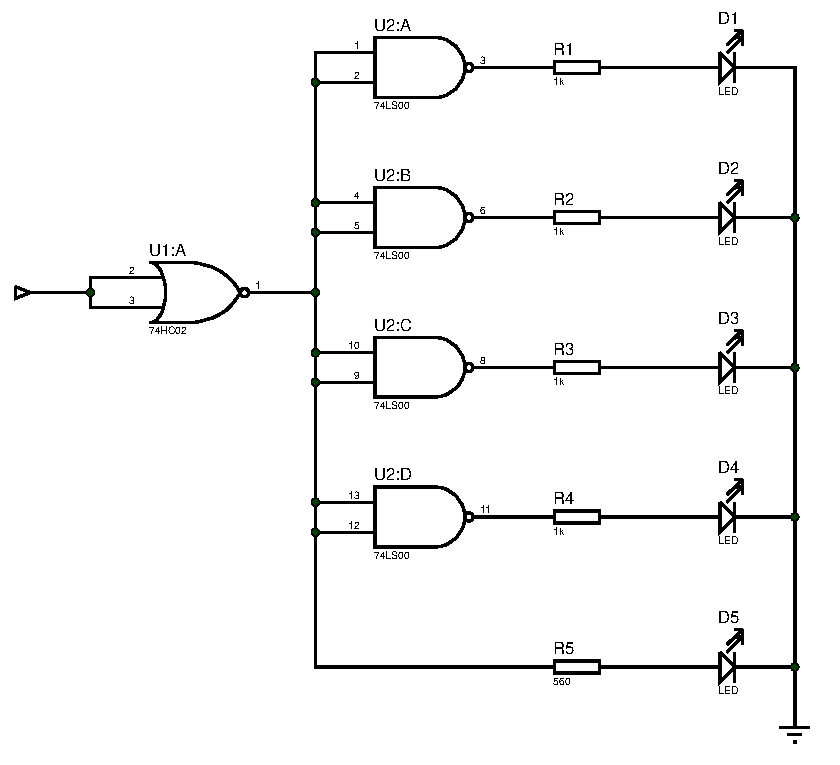
\includegraphics[width=0.7\textwidth]{data/circuitLED}
    \par\end{centering}
    \caption{Circuit load schematic - Made in Proteus 7.8}
\end{figure}

In the following table are the measured times
for the diferent configurations.

\begin{table}[H]
    \begin{center}
    \begin{tabular}{|c|c|c|c|c|}
    \hline
    CASE & $tpd_{L-H}$ & $tpd_{H-L}$ & $t_r$ & $t_f$\\
    \hline \hline
    Without LOAD & 15ns & 5ns & 42ns & 45ns \\ \hline
    Circuit LOAD & 17ns & 5ns & 46ns & 45ns \\ \hline
    Circuit LOAD (100KHz) & 18ns & 4ns & 45ns & 52ns \\ \hline
    Circuit LOAD (100KHz with Capacitors) & 9ns & 4ns & 50ns & 52ns \\ \hline
    \end{tabular}
    \caption{Measured times}
    \end{center}
\end{table}

In the first two cases, it was observed that the 
measured times had no appreciable diferences 
when the gate is charged with 
the external circuit. In the case with the circuit,
 the IC raises its temperature a little. This is
mainly due to the direct charge of the R5 and 
L5 componentes, requesting the IC a current
that is near to the maximum value of $4mA$ per 
output. \newpage
Also the output voltage level decreases
in the case with the circuit charge, compared to 
the case without load, as shown in the next figures. \\

\begin{figure}[H]
    \begin{centering}
    \includegraphics[width=0.49\textwidth]{data/ej4_gate1}
    \includegraphics[width=0.49\textwidth]{data/ej4_circuit}
    \par\end{centering}
    \caption{Voltage levels: CH1 - Gate input, CH2 - Gate output. On the left
    without load, and on the right with the circuit load.}
\end{figure}

In the same circuit, increasing the frecuency 
up to $100KHz$, a decrease was also observed 
in the output voltage level, with a little oscilation 
in the transition from low to high. This is because 
the external ciruit requires more current for 
turning the LED on, wich causes a voltage overshoot
for a short period of time, until the circuit becomes
stable. To absorve this overshoot, a decoupling 
capacitor is placed near the supply pins of the 
IC, with a value of $100nF$. This value is suggested 
by the datasheet of Texas Instruments. Below is shown 
the output change from low to high with the circuit 
at $100KHz$, without and with the capacitor.

\begin{figure}[H]
    \begin{centering}
    \includegraphics[width=0.49\textwidth]{data/ej4_circuit100k1}
    \includegraphics[width=0.49\textwidth]{data/ej4_circuit100kcap}
    \par\end{centering}
    \caption{Transition L-H CH1 - Gate input, CH2 - Gate output. On the left
    without capacitor, and on the right with it.}
\end{figure}
\newpage
Another fact observed is the high noise level
(about 1V) at 
the supply voltage. This was also fixed with the 
decoupling capacitors, as shown below.

\begin{figure}[H]
    \begin{centering}
    \includegraphics[width=0.49\textwidth]{data/ej4_circuit100ksinc}
    \includegraphics[width=0.49\textwidth]{data/ej4_circuit100kconc1}
    \par\end{centering}
    \caption{Supply voltage: CH1 - VCC. On the left
    without capacitor, and on the right with it.}
\end{figure}
